\documentclass[letterpaper,12pt]{article}
\usepackage{tabularx} % extra features for tabular environment
\usepackage{amsmath}  % improve math presentation
\usepackage{float}
\usepackage{pdfpages}

\usepackage{multicol}
\usepackage{graphicx} % takes care of graphic including machinery
\graphicspath{ {./figures/} }
%\usepackage[margin=1in,letterpaper]{geometry} % decreases margins
%\usepackage{cite} % takes care of citations
\usepackage[final]{hyperref} % adds hyper links inside the generated pdf file
\hypersetup{
	colorlinks=true,       % false: boxed links; true: colored links
	linkcolor=blue,        % color of internal links
	citecolor=blue,        % color of links to bibliography
	filecolor=magenta,     % color of file links
	urlcolor =blue         
}
\usepackage[margin = 1in,headsep=0.5cm,headheight=2cm,letterpaper]{geometry} 

\usepackage{fancyhdr}
\pagestyle{fancy}
\lhead{Student 1 : Ahmet Akman 2442366 \\ Student 2: Yusuf Toprak Yıldıran 2444149 \\ Assistant: Onur Selim Kılıç}
\rhead{Date: \today \\ Group: Wednesday Morning - 5} 
%\cfoot{center of the footer!}
\renewcommand{\headrulewidth}{0.1pt}



\begin{document}
\thispagestyle{empty}

\title{Spring 2022 EE214 Experiment 4  \protect\\ Impedance Measurement and Complex Power}
\author{Ahmet Akman 2442366 \protect\\ Yusuf Toprak Yıldıran 2444149 \protect\\ Assistant: Onur Selim Kılıç}
\date{\today}
\maketitle
\tableofcontents
%\begin{abstract}
%abstract
%\end{abstract}
\section{Introduction}
In this experiment, rms values of voltages and currents will be measured then, phase difference between current and voltage will be calculated and complex power and power factor will be measured beside of the the apparent power S,the real power and the reactive power wti the efficiency of the system. Capacitance is aimed to be calculated using voltage and current rms values. Afterwards, 2 different modes of DSO will be used and explained to calculate impedance Z for different frequencies.

\section{Experimental Results and Discussion}
The results of the experiment are discussed in the following steps.
%
\subsection{Step 1}

In this part, circuit in figure 1 is set with \(R_{line}= 100\Omega\) and \(Z_{load}= 560\Omega + j0.1w\) and inductor \(L= 0.1H\).
\begin{figure}[H]
    \centering
    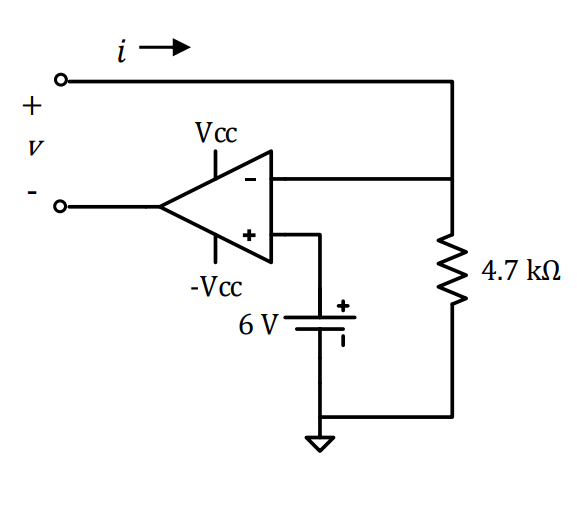
\includegraphics[width = 0.75\textwidth]{1SCH.png}
    \caption{Circuit schematic for the step 1}
\end{figure} 
For the parts below (a-b-c), magnitude of the voltage source is adjusted such that \(V_{load}(t)\) always equals to \(5sin(2000\pi t)\) V. 

\subsubsection{a.}
For this part, rms values of \(V_{in}\), \(V_{line}\), \(V_{load}\), \(i_{load}\) and phase difference between \(V_{load}\) and \(i_{load}\) are measured and recorded in table 1. Rms value of voltages is obtained by using rms measurement tool of DSO and rms current is obtained by measuring the voltage accross \(100\Omega\) resistor. To calculate phase difference, the difference between peak values of the signals is measured in \(\mu s\) and a proportionality with the 1/frequency value is found.


Then, to find \(P_{line}\), \(i_{load}\) is multiplied by \(V_{line}\) ,and power factor is found by using phase difference and found as cos(phase difference(\(54\deg \))) leading. Afterwards, total apparent power on the load \(|S|_{load}\) is found by multiplying \(i_{load}\) with \(V_{load}\) and recorded in table 2 and total real power on the load \(P_{load}\) is found by multiplying \(|S|_{load}\) with power factor(\(cos(54\deg )\)) and recorded in table 2. Then, total reactive power on the load \(Q_{load}\) is found by multiplying \(|S|_{load}\) with \(sin(54\deg )\) and noted in table 2.
\subsubsection{b.}
In this part, 100nF capacitor is connected parallel with the load ,and same measurements and calculations with part a. are made. Then, results are recorded in table 1 and table 2.   
\subsubsection{c.}
For this part, 1\(\mu F\) capacitor is replaced with the 100nF capacitor in part a. and same calculations and measurements are made for this part too.
\subsubsection{d.}

\begin{table}[H]
    \begin{center}
        \caption{Power Measurements}
        \vspace{2mm}
        \begin{tabular}{||c | c | c | c | c | c | c ||} 
            \hline
            Part & \(V_{in}\)\newline (Vrms) & \(V_{line}\)\newline (Vrms) & \(V_{Load}\) \newline (Vrms) &\(i_{Load}\)\newline (mArms) & \(\phi_{Load}\)\newline(degree) &\(\phi_{in}\)\newline(degree)  \\ [0.5ex] 
            \hline\hline
            a. & &  & & & &   \\ 
            \hline
            b. & &  & & & &    \\
            \hline
            c. & &  & & & &   \\ [1ex] 
            \hline
        \end{tabular}
\end{center}
\end{table}


\begin{table}[H]
    \begin{center}
        \caption{Power Calcuations}
        \vspace{2mm}
        \begin{tabular}{||c | c | c | c | c | c ||} 
            \hline
            Part & \(P_{in}\)\newline (mW) & \(P_{line}\)\newline (mW) & \(P_{Load}\) \newline (mW) &\(Q_{Load}\)\newline (mVAR) & \(|S|_{Load}\)\newline(mVA)   \\ [0.5ex] 
            \hline\hline
            a. & &  & & &    \\ 
            \hline
            b. & &  & & &     \\
            \hline
            c. & &  & & &    \\ [1ex] 
            \hline
        \end{tabular}
\end{center}
\end{table}




\begin{table}[H]
  \begin{center}
    \caption{Load Parameters}
    \vspace{2mm}
 \begin{tabular}{||lll|lll|lll||}
    \hline
    \multicolumn{3}{|l|}{Part a. (Load)}                            & \multicolumn{3}{l|}{Part b. Load}                            & \multicolumn{3}{l|}{Part c. Load}                            \\ \hline
    \multicolumn{1}{|l|}{pf} & \multicolumn{1}{l|}{lead/lag} & eff \(\%\) & \multicolumn{1}{l|}{pf} & \multicolumn{1}{l|}{lead/lag} &eff \(\%\)  & \multicolumn{1}{l|}{pf} & \multicolumn{1}{l|}{lead/lag} &eff \(\%\)  \\ \hline
    \multicolumn{1}{|l|}{} & \multicolumn{1}{l|}{} &  & \multicolumn{1}{l|}{} & \multicolumn{1}{l|}{} &  & \multicolumn{1}{l|}{} & \multicolumn{1}{l|}{} &  \\ \hline
    \end{tabular}
\end{center}

\end{table}
\subsection{Step 2}

In this step, circuit in figure 2 is set by adjusting signal generator output to sine wave with 500 Hz frequency and 6 Volt peak to peak voltage value using 1\(\mu F\) capacitor and 1\(k\Omega \) resistor to obtain current. Then, rms value of the voltage V accross capacitor is measured as 1.23 V and rms value of the current passing through capacitor is measured as 3.70 mA. Afterwards, by doing following calculations capacitance C1 is calculated:

\[\frac{V_{rms}}{i_{rms}} = |Z| = \frac{(-j)^2}{w^2C^2}\]
where Z is the impedance and w = \(2\pi (500 Hz)\).  
\[C1 = \frac{i_{rms}}{V_{rms}w}  =  \frac{3.79 mA}{1.23 V . 1000\pi} \approx 0.98x10^{-6} = 0.98 \mu F\]

Then by adjusting LC meter to proper scale, nominal capacitance of the capacitor is measured as 1.03 \(\mu F\)
\begin{figure}[H]
    \centering
    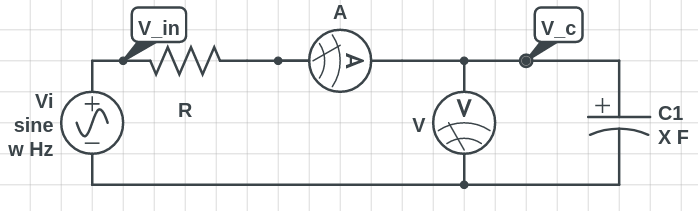
\includegraphics[width = 0.75\textwidth]{2SCH.png}
    \caption{Circuit schematic for the step 2}
\end{figure} 
    
\subsection{Step 3}

In this step, circuit in figure 4 is set with 1.5 kHz and 3 kHz frequency sine wave respectively and 0.1 \(\mu F\) capacitor and 1k\(\Omega \) resistor and 0.1 H inductor are used , then by using 2 different method, impedance Z in figure 3 is measured. 

\subsubsection{First Method}


\subsubsection{Second Method}

\begin{figure}[H]
    \centering
    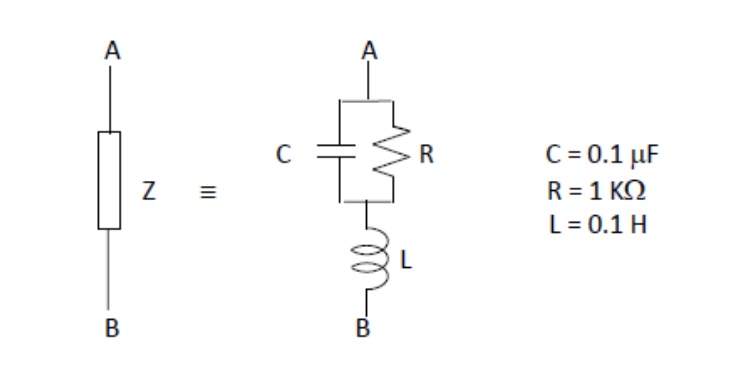
\includegraphics[width = 0.75\textwidth]{3SCH.png}
    \caption{Circuit schematic for the step 3}
\end{figure} 

\begin{figure}[H]
    \centering
    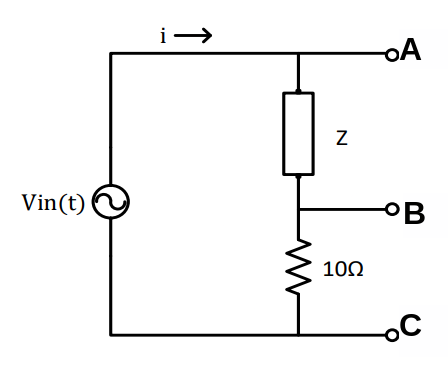
\includegraphics[width = 0.75\textwidth]{3_1SCH.png}
    \caption{Outside circuit schematic for the step 3}
\end{figure} 

\section{Conclusion}
In this experiment, rms values of voltages and currents are measured. Phase difference between current and voltage are calculated and complex power and power factor are measured beside of the the apparent power S,the real power and the reactive power with the efficiency of the system. Capacitance is calculated using voltage and current rms values. Lastly, 2 different modes of DSO are used and explained to calculate impedance Z for 2 different frequencies.


\section*{Appendix A}
\begin{itemize}
    \item PreLab Preparation 3 hours
    \item Experimental Work 2  hours
    \item Report Writing 8 hours
\end{itemize}

\end{document}

%%%%%%%%%%%%%%%%%%%%%%   EXAMPLE TABLE   %%%%%%%%%%%%%%%%%%%%%%%%%%%%%%%%
\begin{table}[H]
\begin{center}
    \caption{Resistance reading by color code convention.}
    \vspace{2mm}
    \begin{tabular}{||c | c | c||} 
        \hline
        Color Order & Value & Tolerance \\ [0.5ex] 
        \hline\hline
        Brown / Black / Red / Gold & 1k\( \Omega \) & \( \% \) 5  \\ 
        \hline
        Yellow / Violet / Red / Gold & 4.7k\( \Omega \) & \( \% \) 5   \\
        \hline
        Brown / Grey / Orange / Gold & 18k\( \Omega \) & \( \% \) 5  \\ [1ex] 
        \hline
    \end{tabular}
\end{center}
\end{table}


%%%%%%%%%%%%%%%%%%%%%%   EXAMPLE IMAGE   %%%%%%%%%%%%%%%%%%%%%%%%%%%%%%%%
\begin{figure}[H]
\centering
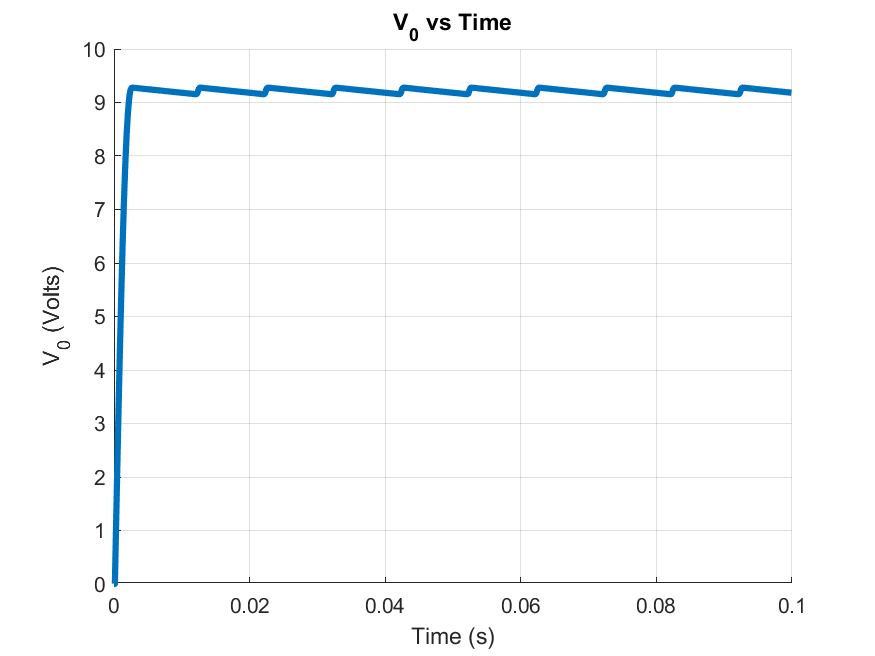
\includegraphics[width = 0.75\textwidth]{5.png}
\caption{Circuit schematic for the step 5}
\end{figure} 

%%%%%%%%%%%%%%%%%%%%%%   EXAMPLE IMAGE FROM PDF   %%%%%%%%%%%%%%%%%%%%%%%%%%%%%%%%
\begin{figure}[H] \centering{
	\includegraphics[scale=0.25]{2a_plot.pdf}}
	\caption{Experiment 2}
\end{figure}
%%%%%%%%%%%%%%%% Deneme Push